\documentclass[a4paper]{article}

% Packages
\usepackage{amsmath}
\usepackage{amssymb}
\usepackage{amsthm}
\usepackage{bold-extra}
\usepackage{fancyhdr}
\usepackage{geometry}
\usepackage{graphicx}
\usepackage{hyperref}
\usepackage{ifthen}
\usepackage[utf8]{inputenc}
\usepackage{multirow}
\usepackage{needspace}
\usepackage{parskip}
\usepackage{stmaryrd}
\usepackage{listings}
\usepackage[T1]{fontenc}
\usepackage{longtable}
\usepackage{comment}
\usepackage{enumerate}
\usepackage{xspace}
\usepackage{textcomp}
\usepackage{array}

\usepackage{tikz}
\usetikzlibrary{automata,positioning,shapes.geometric}
\usepackage{tikzsymbols}
\usepackage{todonotes}

\lstset{language=Java, numbers=left, showstringspaces=false, tabsize=4}
\geometry{a4paper, left=25mm,right=25mm, top=25mm, bottom=25mm}

% check for the existence of commands
\newcommand{\checkfor}[3]{%
  \ifcsname#1\endcsname%
  #2
  \else%
  #3
  \fi%
}

\checkfor{exnumber}{}{\newcommand{\exnumber}{-1}}

\newcommand{\exercisepagebreak}{\checkfor{isexercise}{\pagebreak}{}}
\newcommand{\solutionpagebreak}{\checkfor{isexercise}{}{\pagebreak}}

\setcounter{section}{\exnumber{}}

\numberwithin{equation}{section}
\numberwithin{figure}{section}
\numberwithin{table}{section}
\renewcommand{\qedsymbol}{\textsc{q.e.d.}}
\renewenvironment{proof}[1][\proofname]{{\bfseries #1: }}{\qed}
\newtheoremstyle{defstyle}{10pt}{5pt}{\addtolength{\leftskip}{2\leftmargini}\addtolength{\rightskip}{2\leftmargini}}{-1\leftmargini}{\scshape\bfseries}{:}{\newline}{#1 #2\ifthenelse {\equal {#3}{}} {}{ (\text{\textsc{#3}})}}{}
\newtheoremstyle{thmstyle}{10pt}{5pt}{\addtolength{\leftskip}{2\leftmargini}\addtolength{\rightskip}{2\leftmargini} \slshape}{-1\leftmargini}{\scshape\bfseries}{:}{\newline}{#1 #2\ifthenelse {\equal {#3}{}} {}{ (\text{\textsc{#3}})}}{}
\newtheoremstyle{exstyle}{10pt}{5pt}{\addtolength{\leftskip}{2\leftmargini}\addtolength{\rightskip}{2\leftmargini}}{-1\leftmargini}{\scshape\bfseries}{:}{\newline}{#1 #2\ifthenelse {\equal {#3}{}} {}{ (\text{\textsc{#3}})}}{}
\newtheoremstyle{algostyle}{10pt}{5pt}{\addtolength{\leftskip}{2\leftmargini}\addtolength{\rightskip}{2\leftmargini}}{-1\leftmargini}{\scshape\bfseries}{:}{\newline}{#1\ifthenelse {\equal {#3}{}} { #2}{ \text{\textsc{#3}}}}{}
\theoremstyle{defstyle}
\newtheorem{mydef}{Definition}[section]
\theoremstyle{thmstyle}
\newtheorem{mythm}{Theorem}[section]
\newtheorem{mylem}[mythm]{Lemma}
\newtheorem{myprop}[mythm]{Proposition}
\theoremstyle{exstyle}
\newtheorem{myex}{Example}[section]
\theoremstyle{algostyle}
\newtheorem{myalgo}{Algorithm}

% Define programming and solution environment and only use if enabled
\checkfor{isprog}{
  % Define exercise environment
  \newcounter{exercise}
  \newenvironment{exercise}[1]{\refstepcounter{exercise}\label{ex\theexercise}\section*{Programming Exercise \theexercise \hfill (#1 Points)}}{}
  \checkfor{isexercise}{
    % Programming exercise
    \excludecomment{solution}
    \excludecomment{onlysolution}
    \newenvironment{onlyexercise}{}{}
    \newcommand{\extitle}{Programming Exercise}
  }{
    % Programming solution
    \newenvironment{solution}{\label{sol\theexercise}\subsection*{Solution: \hrulefill}}{}
    \newenvironment{onlysolution}{}{}
    \excludecomment{onlyexercise}
    \newcommand{\extitle}{Programming Solution}
    }
}{
  % Define exercise environment
  \newcounter{exercise}
  \newenvironment{exercise}[1]{\refstepcounter{exercise}\label{ex\theexercise}\section*{Exercise \theexercise \hfill (#1 Points)}}{}
  \checkfor{isexercise}{
    % Theoretical exercise
    \excludecomment{solution}
    \excludecomment{onlysolution}
    \newenvironment{onlyexercise}{}{}
    \newcommand{\extitle}{Exercise Sheet}
  }{
    % Theoretical solution
    \newenvironment{solution}{\label{sol\theexercise}\subsection*{Solution: \hrulefill}}{}
    \newenvironment{onlysolution}{}{}
    \excludecomment{onlyexercise}
    \newcommand{\extitle}{Solution}
  }
}

% Define header
\pagestyle{fancy}
\fancyhf{} % Clear all headers
\setlength{\headsep}{25pt}
\cfoot{\thepage} % Page numbers
\lhead{ % Header-Definition
  % Logo
  \begin{tabular}[b]{l l}
      \multirow{2}{38mm}{
        \raisebox{-3.6mm}[0pt][0pt]{
          \includegraphics[height=14mm]{../i2}
        }
      }
      & Lehrstuhl f{\"u}r Informatik 2 \\
      & Software Modeling and Verification
    \end{tabular}
}
\rhead{ % Header-Definition
  % Course name
  \begin{tabular}[b]{r}
    Compiler Construction 2025\\
    \extitle{} \exnumber
  \end{tabular}
}
\AtBeginDocument{
  \vspace*{-30pt}
  apl.\ Prof.\ Dr.\ Thomas Noll\hfill Daniel Zilken, Roy Hermanns
  \vspace{5mm}
}


\newcommand{\header}[1]{
  % Header
  \begin{center}
    {\huge \textbf{Compiler Construction 2025}}\\
    \vspace*{1\baselineskip}%
    {\huge \textbf{--- \extitle{} \exnumber{} ---}}\\
    \checkfor{isexercise}{
      \vspace*{1\baselineskip}
      \checkfor{isprog}{
        %Upload in Moodle until #1 before the exercise class.
      }{
        Upload in Moodle or hand in until #1 before the exercise class.
      }
    }{}
    \vspace*{1.5\baselineskip}
    \hrule
  \end{center}
}

% Change numbering to (a) and (i)
\renewcommand{\labelenumi}{(\alph{enumi})}
\renewcommand{\labelenumii}{(\roman{enumii})}

% Custom commands
\newcommand{\TODO}[1]{\color{red}\textbf{TODO:} #1\color{black}}

% Macros
\newcommand{\set}[1]{\ensuremath{\left\{ #1 \right\}}}
\newcommand{\Nats}{\ensuremath{\mathbb{N}}}
\newcommand{\Reals}{\ensuremath{\mathbb{R}}}

\newcommand{\PTIME}{\mbox{\rm PTIME}}
\newcommand{\PSPACE}{\mbox{\rm PSPACE}}
\newcommand{\coNP}{\mbox{\rm coNP}}
\newcommand{\NP}{\mbox{\rm NP}}
\newcommand{\poly}{\mbox{\rm poly}}
\newcommand{\coPTIME}{\mbox{\rm coPTIME}}
\newcommand{\coPSPACE}{\mbox{\rm coPSPACE}}
\newcommand{\NPSPACE}{\mbox{\rm NPSPACE}}
\def\EXPTIME{\text{\rm EXPTIME}}
\def\doubleEXPTIME{\text{\rm 2EXPTIME}}

% Lecture specific commands
\renewcommand{\L}{{\cal L}}
\newcommand{\numberone}{\ensuremath{\set{1, \dots, 9}}}
\newcommand{\numberzero}{\ensuremath{\set{0, \dots, 9}}}
\newcommand{\eps}{\ensuremath{\varepsilon}}
\newcommand{\sem}[1]{\llbracket#1\rrbracket}
\newcommand{\la}{\ensuremath{\textsf{la}}}
\newcommand{\fir}{\ensuremath{\textsf{fi}}}
\newcommand{\first}{\ensuremath{\textsf{first}}}
\newcommand{\fo}{\ensuremath{\textsf{fo}}}
\newcommand{\follow}{\ensuremath{\textsf{follow}}}
\newcommand{\cyl}[1]{\ensuremath{\mathit{Cyl}(#1)}}
\newcommand{\icompiler}[0]{\texttt{i2Compiler}}
\newcommand{\while}[0]{\textit{WHILE}\xspace}



%for fancy definitions in ex5
\usepackage{mdframed}
\usepackage{csquotes}

\begin{document}

\header{November 16th}

\begin{onlysolution}
  \begin{center}
    \includegraphics[scale=0.5]{xkcd_formal_languages}

    [audience looks around] ``What just happened?'', ``There must be some context we're missing'' \\[0.5em]

    \scriptsize Credit: \href{https://xkcd.com/1090/}{https://xkcd.com/1090/}
  \end{center}
\end{onlysolution}

\section*{General Remarks}
\begin{itemize}
  %
  \item If you have questions regarding the exercises, feel free to write us an email:
  \[\text{   \href{mailto:cc22@i2.informatik.rwth-aachen.de}{cc22@i2.informatik.rwth-aachen.de}}
  \]
  %
  %
  \item Exercises are \emph{optional}, i.e., not required for admission to exams. However, corrections to students’ solutions are provided as annotations to the submissions.
  %
  \item You can hand in your solution to the tasks digitally in the Moodle room. Alternatively, you can hand in your solution to the tasks at our chair in the corresponding box or before the exercise class.
  %
  \item Please hand in your solutions in \emph{groups of four} and hand in only one solution per group. You can use the forum in this Moodle room to find group members.
\end{itemize}

%%%%%%%%%%%%%
% Dot not use this exercise anymore please! It only has problems...
%%%%%%%%%%%%%

\begin{exercise}{40}
%\textit{Note: This exercise has been changed slightly in the solution in order to accommodate remarks from the exercise class.}\par
        On July 20, 2016 the popular website \href{https://stackoverflow.com}{stackoverflow.com} experienced an unexpected outage due to a malformed post
that caused its backtracking Regex engine to consume extraordinary high CPU time.\footnote{Details are provided at \url{http://stackstatus.net/post/147710624694/outage-postmortem-july-20-2016}}
This is an example of a \emph{regular expression denial-of-service} (ReDoS) attack:
An attacker tries to paralyze an application by feeding it with input strings that exhibit high computational complexity.\par

In this exercise, we have a closer look at "attack strings" for the word problem of an NFA $\mathfrak{A}$ (\enquote{given $w$, is $w \in L(\mathfrak{A})$?}) without $\epsilon$-transitions. We assume that our algorithm for solving the word problem  is very naive and explores each possible run of an NFA on a word $w$ individually.
%for a given sequence of NFAs $\mathfrak{A}_1, \ldots, \mathfrak{A_n}$ over the alphabet $\Omega$ instead of regular expressions $\alpha_1, \ldots, \alpha_n \in \textit{RE}_{\Omega}$. 

We call an NFA $\mathfrak{A}$ \emph{vulnerable} if and only if the worst-case complexity of this naive algorithm is exponential in the length of the input word $w$.

\begin{enumerate}[(a)]
  \item Provide an example of a vulnerable NFA $\mathfrak{A}$ and, for each $k \geq 1$, an input string $w_n$ of length $|w_n| = n \geq k$ such that the runtime of the naive algorithm on $w_n$ is exponential in $n$.

  \item A \emph{path} in an NFA $\mathfrak{A} = (Q,\Omega,\delta,q_0,F)$ is a sequence of transitions $\pi = (q_1,\ell_1,q_2)\ldots(q_{m-1},\ell_{m-1},q_m)$ such that $q_i \in Q$, $\ell_i \in \Omega$, and $q_{i+1} \in \delta(q_i,\ell_i)$. Moreover, we set $\textit{labels}(\pi) = \ell_1 \ldots \ell_{m-1}$.

    Show that an NFA $\mathfrak{A}$ is vulnerable if there exists a state $q$ and two distinct paths $\pi_1$, $\pi_2$ such that
            \begin{enumerate}[(i)]
              \item both $\pi_1$ and $\pi_2$ start and end at state $q$,
              \item $\textit{labels}(\pi_1) = \textit{labels}(\pi_2)$,
              \item there is a path $\pi_p$ from initial state $q_0$ to $q$, and
              \item there is a path $\pi_s$ from $q$ to a state $q_r \notin F$.
            \end{enumerate}
  \item Sketch a procedure that takes an NFA $\mathfrak{A}$ and one of its states $q$ as an input and checks whether $\mathfrak{A}$ is vulnerable using the criterium from \textbf{(b)} for the given state $q$.
  \end{enumerate}
\end{exercise}


\begin{solution}
\begin{enumerate}[(a)]
    \item Let $\Omega = \{a,b\}$. For each $k \geq 1$, we choose the input string $w_n = a \cdot a^{2k} \cdot b$ with length $|w_n| = 2k+2 \geq k$, and the following NFA:

    \begin{center}
          \begin{tikzpicture}[->,shorten >=1pt,auto,thick,node distance=2.5cm]
            \tikzstyle{every state}=[draw=black,text=black, minimum width = .7cm]

            \node[state, initial, initial text=] (0) at (0,0) {0};
            \node[state, accepting] (1) at (2,0) {1};
            \node[state] (2) at (4,0) {2};

            \path[every node/.style={font=\sffamily\small}]
              (0) edge node[above] {$a$} (1)
              (0) edge[bend right]  node[below left] {$b$} (2)
              (1) edge node[above] {$b$} (2)
              (1) edge[bend right] node[above] {$a$} (0)
              (1) edge[loop above] node[above] {$a$} (1)
            ;
          \end{tikzpicture}
        \end{center}

    The NFA is vulnerable.
    From state $1$ and input $aa$ two possible paths $1 \overset{a}{\rightarrow} 0 \overset{a}{\rightarrow} 1$ and $1 \overset{a}{\rightarrow} 1 \overset{a}{\rightarrow} 1$ are possible.
    That means for input $(aa)^k$ there are $2^k$ possible paths which must be considered in the worst-case.
    As the input $w_n$ is not accepted (because of suffix $b$) we have to consider all $2^k$ many paths.

    \item Consider a string of the form $w_p \cdot w^k \cdot w_s$, where $w_p = \textit{labels}(\pi_p)$, $w = \textit{labels}(\pi_1) = \textit{labels}(\pi_2)$, $w_s = \textit{labels}(\pi_s)$, and $k \geq 1$.

    We show for each $k \geq 1$ that there are at least $2^{k}$ possible runs of $\mathfrak{A}$ on $w_p \cdot w^{k}$ that end up in $q$. By induction on $k$.

    \textbf{Induction base.} For $k=1$, we know from (iii) that $\pi_p$ leads to $q$.
    By (i) this means that $\pi_p \cdot \pi_1$ and $\pi_p \cdot \pi_2$ lead to $q$.
    Moreover, by (ii), we have $\textit{labels}(\pi_p \cdot \pi_1) = \textit{labels}(\pi_p \cdot \pi_2) = w_p \cdot w$.
    Hence, there are at least two runs of $\mathfrak{A}$ on $w_p \cdot w$ that end up in $q$.

    \textbf{Induction hypothesis.}
    Assume for an arbitrary, but fixed $k \geq 1$ that there are at least $2^{k}$ possible runs of $\mathfrak{A}$ on $w_p \cdot w^{k}$ that end up in $q$.

    \textbf{Induction step.}
    Consider the word $w_p \cdot w^{k+1}$.
    By I.H. there are at least $2^{k}$ possible runs of $\mathfrak{A}$ on $w_p \cdot w^{k}$ that end up in $q$.
    Since $\textit{labels}(\pi_1) = \textit{labels}(\pi_2) = w$ (by (ii)), we know from (i) that for each of these runs $\pi$
    there are two runs of $\mathfrak{A}$ on $w_p \cdot w^{k+1}$ that end up in $q$.
    More precisely, these runs are $\pi \cdot \pi_1$ and $\pi \cdot \pi_2$.
    Hence there are at least $2 \cdot 2^{k} = 2^{k+1}$ runs of $\mathfrak{A}$ on $w_p \cdot w^{k+1}$ that end up in $q$.

    Now, by (iv) we know that there are at least $2^{k}$ runs of $\mathfrak{A}$ on $w_p \cdot w^{k} \cdot w_s$ that are \emph{rejected} by $\mathfrak{A}$.
    Hence, in the worst case, the naive algorithm has to consider each of these $2^{k}$ possible runs.
    In other words, the runtime of the naive algorithm is exponential in the input string.

    \textbf{Remark:}
    In the case of our FLM analysis these four conditions are not sufficent. We also need a fifth condition
    \begin{enumerate}[(v)]
        \item $q \in P$.
    \end{enumerate}
    This condition ensures that state $q$ is productive. Otherwise the Backtracking NFA could abort early on for unproductive states as it will never reach an accepting state again.

    \item Assume that $\mathfrak{A} = (Q,\Omega,\delta,q_0,F)$ and $q \in Q$.
    We construct a new NFA $\mathfrak{A}_{\text{evil}}$ that accepts all possible attack strings for state $q$.
    If the language of $\mathfrak{A}_{\text{evil}}$ is non-empty then $\mathfrak{A}$ is vulnerable for $q$.
    Our construction works as follows:


    \begin{align*}
      & \mathfrak{A}_{\text{evil}} ~=~ \texttt{empty NFA} \\
      & \texttt{for}~ q_1,q_2 \in \delta(q,\ell) ~\texttt{and}~ q_1 \neq q_2~\texttt{do} \\
      & \qquad \mathfrak{A}_1 ~=~ \mathfrak{A}_{\texttt{loop}}(q,\ell,q_1) \\
      & \qquad \mathfrak{A}_2 ~=~ \mathfrak{A}_{\texttt{loop}}(q,\ell,q_2) \\
      & \qquad \mathfrak{A}_p ~=~ (Q,\Omega,\delta,q_0,\{q\}) \\
      & \qquad \mathfrak{A}_s ~=~ (Q,\Omega,\delta,q,F) \\
      & \qquad \mathfrak{A}_{\text{evil}} ~=~ \mathfrak{A}_{\text{evil}} ~\cup~ \left( \mathfrak{A}_p \cdot (\mathfrak{A}_1 \cap \mathfrak{A}_2)^{+} \cdot \overline{\mathfrak{A}_s} \right) \\
      & \texttt{return}~\mathfrak{A}_{\text{evil}}
    \end{align*}
    In this construction, the automaton $\mathfrak{A}_{\texttt{loop}}(q,\ell,q_i)$, $i \in \{1,2\}$, is given by
    \[ (Q \cup \{q'\}, \Omega, \delta \cup \{(q',\ell,q_i)\}, q', \{q\})~, \]
    where $q'$ is a fresh state.
\end{enumerate}

\end{solution}


\begin{exercise}{30}
 Consider the context-free grammar $G$ given by the following rules:
 \begin{align*}
    S  ~\to~ a ~|~ (\,S\,) ~|~ S \cdot S ~|~ S + S ~|~ -S
 \end{align*}
 \begin{enumerate}[(a)]
  \item Provide a leftmost analysis of the string $a \cdot (-a + (a))$.
  \item Provide a rightmost analysis of the string $a \cdot (-a + (a))$.
  \item Prove or disprove: $G$ is unambiguous.
 \end{enumerate}
\end{exercise}

\begin{solution}
 We enumerate the rules from left to right starting with $1$.

\begin{enumerate}[(a)]
 \item
 \begin{align*}
                         & S \\
   ~\Rightarrow_{l}^{3}~ & S \cdot S \\
   ~\Rightarrow_{l}^{1}~ & a \cdot S \\
   ~\Rightarrow_{l}^{2}~ & a \cdot (\,S\,) \\
   ~\Rightarrow_{l}^{5}~ & a \cdot (\,-S\,) \\
   ~\Rightarrow_{l}^{4}~ & a \cdot (\,-S + S\,) \\
   ~\Rightarrow_{l}^{1}~ & a \cdot (\,-a + S\,) \\
   ~\Rightarrow_{l}^{2}~ & a \cdot (\,-a + (\,S\,)\,) \\
   ~\Rightarrow_{l}^{1}~ & (\,-a + (\,a\,)\,)
 \end{align*}
 Hence, a leftmost analysis of $a \cdot (-a + (a))$ is $z_{l} = 31254121$.

 \item
 \begin{align*}
                         & S \\
   ~\Rightarrow_{r}^{3}~ & S \cdot S \\
   ~\Rightarrow_{r}^{2}~ & S \cdot (\,S\,) \\
   ~\Rightarrow_{r}^{4}~ & S \cdot (\,S + S\,) \\
   ~\Rightarrow_{r}^{2}~ & S \cdot (\,S + (\,S\,)\,) \\
   ~\Rightarrow_{r}^{1}~ & S \cdot (\,S + (\,a\,)\,) \\
   ~\Rightarrow_{r}^{5}~ & S \cdot (\,-S + (\,a\,)\,) \\
   ~\Rightarrow_{r}^{1}~ & S \cdot (\,-a + (\,a\,)\,) \\
   ~\Rightarrow_{r}^{1}~ & a \cdot (\,-a + (\,a\,)\,)
 \end{align*}
 Hence, a rightmost analysis of $a \cdot (-a + (a))$ is $z_{r} = 32421511$.

 \item
 $G$ is ambiguous. For example, there exist two leftmost analysis for the word from part (a) $a \cdot (-a + (a))$, namely
 $z_1 = 31254121$ and $z_2 = 31245121$.
\end{enumerate}

\end{solution}

%\begin{exercise}{50}
      Complete the correctness proof of %Theorem~5.15
      Theorem~6.3 by showing the direction omitted in the lecture.
      %
      More precisely, let $G = \langle N, \Sigma, P, S \rangle \in \textnormal{CFG}_{\Sigma}$ and $NTA(G)$ as in %Definition~5.13.
      Definition~6.1.
      %
      Show that for each $w \in \Sigma^{*}$ and $z \in [p]^{*}$ it holds that
      \begin{align*}
         (w,S,\varepsilon) ~\vdash^{*}~ (\varepsilon,\varepsilon,z)  \quad\text{implies}~\quad z~\text{is a leftmost analysis of}~w.
      \end{align*}
\end{exercise}

\begin{solution}
We prove a stronger statement: For all $z \in [p]^*, w =uv, \alpha = uA\beta$ with $A \in N \cup \{\epsilon\}$,

$$(uv, \alpha, y) \vdash^* (\varepsilon, \varepsilon, yz) \text{ implies } \alpha \to_l^z w ~.$$

The proof is by induction over $n = |z|$:\\

$\bf{n=0}$: then $\alpha = w$ as there may only be matching steps and thus
$$(w, w, y) \vdash^* (\varepsilon, \varepsilon, y) \text{ implies } w \to_l^\varepsilon w$$

$\bf{n \to n+1}$: for $z = iz'$ we know from induction that if
	$(w', \alpha', y') \vdash^* (\varepsilon, \varepsilon, y'z')$
	then $\alpha' \to_l^{z'} w'$.\\

	Let $\alpha = uA\beta$, $w = uv$, where $u, v \in \Sigma^*$	and let $\pi(i) = A \to \gamma$.
    Then
    $$(w, \alpha, y) = (uv, uA\beta, y) \vdash^* (v, A\beta, y) \vdash (v, \gamma\beta, yi)$$
    We know from the premise of the induction hypothesis that $(w', \alpha', y') \vdash^* (\varepsilon, \varepsilon, y'z')$.\\
    Let $w'=v$, $\alpha'=\gamma\beta$, $y'=yi$.
    Then
    $$(v, \gamma\beta, yi) \vdash^* (\varepsilon, \varepsilon, yiz')$$

The above implies:
\begin{center}
$\begin{array}{rlrlll}
&& \alpha' &\to_l^{z'}& w' & \text{(from induction hypothesis)}\\
&& \gamma\beta &\to_l^{z'}& v & (\alpha'=\gamma\beta, w'=v) \\
&& u\gamma\beta &\to_l^{z'}& uv = w & \\
\alpha = uA\beta &\to^i_l& u\gamma\beta
 &\to_l^{z'}& uv = w & (\text{as }\pi(i) = A \to \gamma) \\
\multicolumn{3}{r}{\alpha = uA\beta} &\to_l^{iz'=z}& uv = w &
\end{array}$
\end{center}
\end{solution}


\begin{exercise}{30}
%
In this task, we define a context-free grammar to specify all valid sequences of \emph{tokens} for a simplified variant of our \emph{While} language. More formally, your task is to give $G \in \textsf{CFG}_\Sigma$ where $\Sigma$
%
is the alphabet of tokens given by the table at the end of this exercise and
%
\begin{align*}
   L(G) = \big\{ w = T_1\ldots T_n \in \Sigma^* ~\mid~ & (T_1,\ldots,T_n)~\text{is the analysis of some syntactically correct program $c$}  \big\}~.
\end{align*}
%
For simplicity, we assume that all variables and constants are of type INT, and that all comments and blanks are ignored. Furthermore, every program must end with an eof. Consider the following program as an example:
%
  \begin{center}
	\begin{tabular}{c}
		\begin{lstlisting}
		/* test program */
		int n = 10;
		while ( n > 0 ) {
		 n = n - 1;
		}
		eof
		\end{lstlisting}
	\end{tabular}
\end{center}
%
The corresponding lexical analysis is given by
%
\begin{align*}
    (&\text{INT}, \text{ID}, \text{ASSIGN},\text{NUMBER},\text{SEM},\text{WHILE},\text{LBRAC},\text{ID},\\
    &\text{GT},\text{NUMBER},\text{RBRAC},\text{LCBRAC},\text{ID},\text{ASSIGN},\text{ID},\text{MINUS},\text{NUMBER},\text{SEM},\text{RCBRAC}, \text{EOF})~.
\end{align*}
%
\emph{Hint: It might be a good idea to design your grammar in a modular fashion, i.e., to introduce nonterminals like program, statement, guard,... .}

\newcolumntype{L}{>{\ttfamily}l}
\begin{longtable}{Ll}
	\hline
	lexeme ~~~~~~~              & token  \\
	\hline
	int          & INT \\
	while      & WHILE \\
	if         & IF \\
	else       & ELSE \\
	
	==         & EQ \\
	<          & LT \\
	>          & GT \\
	
	!          & NOT \\
	\&\&       & AND \\
	||         & OR \\
	
	+          & PLUS \\
	-          & MINUS \\
	*          & TIMES \\
	/          & DIV\\
	\%          & MOD \\
	
	;          & SEM \\
	=          & ASSIGN \\
	(          & LBRAC \\
	)          & RBRAC \\
	\{         & LCBRAC \\
	\}         & RCBRAC\\
	
	0 $\mid ($- $\mid \varepsilon)\{$1$\ldots$9$\}\{$0$\ldots$9$\}^\ast$ & NUMBER \\
	$\{$a$\ldots$zA$\ldots$Z\_$\}\{$a$\ldots$zA$\ldots$Z0$\ldots$9\_$\}^\ast$ & ID \\
	
	eof & EOF \\
	
	\hline
\end{longtable}


\end{exercise}


\begin{solution}
	%
\begin{center}
	\begin{tabular}{lll}
		start       &$\to$ & program EOF\\
		program     &$\to$ & statement program $\mid$ statement\\
		statement   &$\to$ & declaration SEM $\mid$ assignment SEM $\mid$ branch $\mid$ loop $\mid$ out SEM\\
		declaration &$\to$ & INT ID $\mid$ INT ID ASSIGN expr\\
		assignment  &$\to$ & ID ASSIGN expr $\mid$ ID ASSIGN READ LBRAC RBRAC\\
		out         &$\to$ & WRITE LBRAC expr RBRAC $\mid$ WRITE LBRAC STRING RBRAC\\
		branch      &$\to$ & IF LBRAC guard RBRAC LCBRAC program RCBRAC $\mid$\\
		&      & IF LBRAC guard RBRAC LCBRAC program RCBRAC\\
		&      & ELSE LCBRAC program RCBRAC\\
		loop        &$\to$ & WHILE LBRAC guard RBRAC LCBRAC program RCBRAC\\
		expr        &$\to$ & NUMBER $\mid$ ID $\mid$ subexpr\\
		subexpr     &$\to$ & expr PLUS expr $\mid$ expr MINUS expr $\mid$ expr TIMES expr $\mid$ expr DIV expr\\
		&      & $\mid$ expr MOD expr\\
		guard       &$\to$ & relation $\mid$ subguard $\mid$ NOT LBRAC guard RBRAC\\
		subguard    &$\to$ & guard AND guard $\mid$ guard OR guard\\
		relation    &$\to$ & expr LT expr $\mid$ expr LEQ expr $\mid$ expr EQ expr $\mid$ expr LT expr $\mid$ expr GT expr
	\end{tabular}
\end{center}
\end{solution}

%\begin{exercise}{??}
Consider the following grammar $G$:
    \begin{align*}
        S ~\to~ & c S \mid A a \\
        A ~\to~ & a A c \mid B c \\
        B ~\to~ & b D \\
        C ~\to~ & a C a \mid \epsilon \\
        D ~\to~ & a D \mid c
    \end{align*}

\begin{enumerate}[(a)]
    \item Reduce the grammar $G$ to the grammar $G'$.
    \item Compute the first ($\first$) sets for all nonterminal symbols in $G'$.
    \item Compute the follow ($\follow$) sets for all nonterminal symbols in $G'$.
    \item Does $G' \in LL(1)$ hold? Justify your answer.
    \item Could we prove or disprove $G \in LL(1)$ using Theorem 6.9 without the reduce step? What can you conclude about the validitity of Lemma 6.11 with respect to potentially non-reduced, context-free grammars?
\end{enumerate}
\end{exercise}

\begin{solution}
\begin{enumerate}
\item $C$ is not reachable, thus we remove $C$ and receive the reduced grammar $G'$:
    \begin{align*}
        S ~\to~ & c S \mid A a \\
        A ~\to~ & a A c \mid B c \\
        B ~\to~ & b D \\
        D ~\to~ & a D \mid c
    \end{align*}
\item The first sets are as follows:
    \begin{align*}
        \first(S) &= \set{a, b, c} \\
        \first(A) &= \set{a, b} \\
        \first(B) &= \set{b} \\
        \first(D) &= \set{a, c}
    \end{align*}

\item The follow sets are as follows:
\begin{align*}
    \fo(S) &= \set{\varepsilon} \\
    \fo(A) &= \set{a,c} \\
    \fo(B) &= \set{c} \\
    \fo(D) &= \set{c} \\
\end{align*}

\item $G' \in LL(1)$ does hold.
    We compute all $\la$ sets:
    \begin{align*}
        \la(S \rightarrow c S ) &= \{ c \}\\
        \la(S \rightarrow A a ) &= \{ a, b \}\\
        \cline{1-2}
        \la(A \rightarrow a A c ) &= \{ a \}\\
        \la(A \rightarrow B c ) &= \{ b \}\\
        \cline{1-2}
        \la(B \rightarrow b D ) &= \{ b \}\\
        \cline{1-2}
        \la(D \rightarrow a D ) &= \{ a \}\\
        \la(D \rightarrow c ) &= \{ c \}\\
    \end{align*}
    Since the $\la$ sets are disjoint for every non-terminal symbol, we have $G' \in LL(1)$.

\item We can still use Theorem 6.9: We calculate the $\first$, $\fo$ and $\la$ sets for $C$:
    \begin{align*}
        \first(C) &= \{ a, \epsilon \}\\
        \fo(C) &= \emptyset\\
        \cline{1-2}
        \la(C \rightarrow a C a) &= \{ a \}\\
        \la(C \rightarrow \epsilon) &= \emptyset
    \end{align*}
    Since $\la(C \rightarrow a C a) \cap \la(C \rightarrow \epsilon) = \emptyset$ we can still conclude that the grammar is $LL(1)$.\\
    However, if we use Lemma 6.11, we get the following calculation:
        \begin{align*}
        \first(C) &= \{ a, \epsilon \}\\
        \fo(C) &= \{ a \}\\
        \cline{1-2}
        \la(C \rightarrow a C a) &= \{ a \}\\
        \la(C \rightarrow \epsilon) &= \{ a \}
    \end{align*}
    Now we have $\la(C \rightarrow a C a) \cap \la(C \rightarrow \epsilon) = \{ a \}$, which would mean that $G$ is \textbf{not} in $LL(1)$, thus it is really required to reduce $G$ for the algorithm.
\end{enumerate}
\end{solution}


%\begin{exercise}{??}
Theorem~6.9 provides an alternative characterization of $LL(1)$ grammars as given in Definition~6.3. We now want to see whether Theorem~6.9 can be generalized to $LL(k)$ grammars for all $k\in \Nats$. First, recap Definition~6.3:

\begin{mdframed}[linecolor=cyan, linewidth=2pt, topline=false, rightline=false, bottomline=false, skipabove=10pt, skipbelow=10pt]
A context free grammar $G = \langle N, \Sigma, P, S \rangle$ is in $LL(k)$ if and only if for all leftmost derivations of the form
\begin{align*}
    S ~\Rightarrow_{l}^{*}~ wA\alpha \begin{cases}
                                    \Rightarrow_{l} w\beta\alpha \\
                                    \Rightarrow_{l} w\gamma\alpha
                                  \end{cases}
\end{align*}
such that $\beta \neq \gamma$, it follows that $\first_k(\beta\alpha) \cap \first_k(\gamma\alpha) = \emptyset$.
\end{mdframed}

Second, we generalize Theorem 6.9 from $LL(1)$ to $LL(k)$ as follows:

\begin{mdframed}[linecolor=cyan, linewidth=2pt, topline=false, rightline=false, bottomline=false, skipabove=10pt, skipbelow=10pt]
Let $k\in \Nats$. Then $G$ is in $LL(k)$ if and only if for all pairs of rules $A \to \beta \mid \gamma \in P$ (where $\beta \neq \gamma$) we have
\begin{align*}
    \la_k(A \to \beta) \,\cap\, \la_k(A \to \gamma) ~=~ \emptyset~,
\end{align*}
where $\la_k(A \to \beta) = \first_k(\beta \cdot \follow_k(A))$
\end{mdframed}

Prove or disprove: Our modified version of Theorem~6.9 is sound for all $k\in\mathbb{N}$.
\end{exercise}

\begin{solution}
We disprove this statement by showing that the following grammar is $LL(2)$ according to the first, but not to the second characterization:

$G$ is given by the production rules:
  \begin{align*}
    S ~\to~ & aAab ~|~ bAbb \\
    A ~\to~ & a ~|~ \varepsilon
  \end{align*}
We compute the first, follow and lookahead sets for $k=2$ of $G$:
\begin{itemize}
\item $\textrm{first}_2(S) = \{aa, ba, bb\}$
\item $\textrm{first}_2(A) = \{a, \varepsilon\}$
\item $\textrm{follow}_2(S) = \{\varepsilon\}$
\item $\textrm{follow}_2(A) = \{ab, bb\}$\\
\item $\la_2(S \to aAab) = \{aa\}$
\item $\la_2(S \to bAbb) = \{ba, bb\}$
\item $\la_2(A \to a) = \{aa, ab\}$
\item $\la_2(A \to \varepsilon) = \{ab, bb\}$
\end{itemize}
Since $\la_2(A \to a) \cap \la_2(A \to \varepsilon) = \{ab\} \neq \emptyset$ the grammar $G$ is \textbf{not in} $LL(2)$ according to the second definition.\\
\\
Now we check all leftmost derivations as in the first definition:
\begin{itemize}
\item $S \to_l aAab$, $S \to_l bAbb$\\
$\textrm{first}_2(aAab) \cap \textrm{first}_2(bAbb)
= \{aa\} \cap \{ba, bb\} = \emptyset$ \\

\item $S \to_l a\,Aab \to_l a\,aab$, $S \to_l a\,Aab \to_l a\,ab$\\
$\textrm{first}_2(aab) \cap \textrm{first}_2(ab)
= \{aa\} \cap \{ab\} = \emptyset$ \\

\item $S \to_l b\,Abb \to_l b\,abb$, $S \to_l b\,Abb \to_l b\,bb$\\
$\textrm{first}_2(abb) \cap \textrm{first}_2(bb)
= \{ab\} \cap \{bb\} = \emptyset$
\end{itemize}

Thus, the grammar $G$ is \textbf{in} $LL(2)$ according to the first definition. \\
\end{solution}



\end{document}
